%!TEX root = ../thesis.tex
%*******************************************************************************
%*********************************** First Chapter *****************************
%*******************************************************************************

\chapter{Results}  %Title of the First Chapter
\label{chapterresults}

\ifpdf
\graphicspath{{Chapter5/Figs/Raster/}{Chapter5/Figs/PDF/}{Chapter5/Figs/}}
\else
\graphicspath{{Chapter5/Figs/Vector/}{Chapter5/Figs/}}
\fi

One of the aims of this study was to check how the designed impedance device detects plethysmography signals. Another objective was to verify how what changes in plethysmography waveform are detectable by the instrument. As described in chapter \ref{chapterdesign} the designed device is capable of providing electrical signals comparable to the impedance of the body section. The iPG instrument provides output ports of the current driven into the patient, impedance readings and plethysmography waveform of volume under test. In chapter \ref{chapterprocedure}, these signals were converted from voltage representations into readable units such as impedance values in ohms (\si{\ohm}) and currents (\si{\ampere}. Then, a GUI provided analysis of the signals, as well as post-processing options. Last, the data was converted into measurements of blood flow.

\todo{Maybe to describe in a single line about the experimental procedure}

This chapter describes the results obtained from the experimental work. It will show the device capability of detecting impedance baseline signals and plethysmography waveforms. Later, an outline of the numeric results during occlusion will be explained when compared to the additional instruments used during the study. 

\todo{First report the volume measured and the impedance correlated}


%%********************************** % Section 5.1 ******************************************
\section{Physiological measurements}
\label{section5.1}
In the beginning of the research, from the participants recruited population characteristics, physiological measurements and blood pressure values were taken \todo{reference to section that includes a figure of the arm with the measurements position}. In total three female and six male took part of the study. Their age were between \SIrange{23}{37}{year-old} (mean $29.12 \pm 4.94$). The table \ref{tbl:physiological} overviews the data and measurements collected from the participants previous the experiment.

\begin{table}[htbp] %tbl:physiologica
	\caption{Participants' forearm measurements and initial volume.}
	\label{tbl:physiological}
	\centering
	\begin{tabular}{lcc|ccc}
		\toprule
		              &              &              &         \multicolumn{3}{c}{\textbf{Dimensions [\si{\cm}]}}         \\
		              & \textbf{Age} & \textbf{Sex} & \textbf{Arm length} & \textbf{Shoulder} & \textbf{Total length} \\
		              &              &              &                     &  \textbf{to heart}   &  					 \\ \midrule
		Participant 1 &      26      &     Male     &         80          &          26          &          106          \\
		Participant 2 &      23      &    Female    &         66          &          24          &          90           \\
		Participant 3 &      27      &    Female    &         74          &          24          &          98           \\
		Participant 4 &      37      &     Male     &         68          &          24          &          92           \\
		Participant 5 &      29      &    Female    &         62          &          24          &          86           \\
		Participant 6 &      36      &     Male     &         70          &          24          &          94           \\
		Participant 7 &      29      &     Male     &         73          &          23          &          96           \\
		Participant 8 &      26      &     Male     &         69          &          23          &          92           \\ \bottomrule
	\end{tabular}
\end{table}

From the sensing electrodes position is possible to estimate the segments volume by measuring the distance between electrodes ($l$), circumference in each electrode (C$_1$ and C$_2$).  This measuring method is not very accurate (see section \todo{Add reference to a section where how measurements were taken}) but at least guesses a picture of the initial volume of the conductive segment. Table \ref{tbl:measurments} shows the dimensions of the participants forearm between the sensing electrodes and the segment's volume calculate from equation \ref{eq:v_e}.

\begin{table}[htbp] %tbl:measurments
	\caption{Participants' forearm measurements and initial volume.}
	\label{tbl:measurments}
	\sisetup{separate-uncertainty=true}
	\centering
	\begin{tabular}{lcccccc	S[table-format=2.2]@{\,\( \pm \)\,}S[table-format=1.2]}
		\toprule
		&  \textbf{L [\si{\cm}]}   &  \textbf{C$_1$ [\si{\cm}]}  &  \textbf{C$_2$ [\si{\cm}]}  &   \textbf{Ve [\si{\cubic\cm}]} \\\midrule
		Participant 1 & 14.8 & 17.5 & 27.5 & 606.05 \\
		Participant 2 & 11.0 & 15.0 & 20.0 & 269.90 \\
		Participant 3 & 13.0 & 19.0 & 26.5 & 540.27 \\
		Participant 4 & 10.0 & 17.5 & 25.0 & 363.07 \\
		Participant 5 & 10.0 & 17.5 & 23.5 & 336.81 \\
		Participant 6 & 11.0 & 18.5 & 27.0 & 458.32 \\
		Participant 7 & 13.5 & 15.0 & 23.0 & 393.55 \\
		Participant 8 & 11.5 & 17.0 & 23.5 & 378.49 \\ \bottomrule
	\end{tabular}
\end{table}

Executing a mechanical occlusion of the upper arm limits the blood flow towards the forearm. As detailed in the chapter  \ref{chapterprocedure}, blood pressure was taken before the study began. The mean systolic and diastolic pressures were \SI{116.25}{\mmHg}$\pm$\SI{13.66}{\mmHg} and \SI{72.75}{\mmHg}$\pm$\SI{7.23}{\mmHg} respectively. Venous occlusion took place below systolic pressure (mean \SI{55}{\mmHg}$\pm$\SI{8.01}{\mmHg}), partial arterial pressure calculated from equation \ref{eq:meanpressure} was about  \SI{94.63}{\mmHg}$\pm$\SI{10.21}{\mmHg} and total occlusion was around \SI{136.25}{\mmHg}$\pm$\SI{13.67}{\mmHg}. Table \ref{tbl:occlusions} details the blood pressures recorded.

\begin{table}[htbp] %tbl:occlusions
	\caption{Participants' initial blood pressure and levels for venous, partial arterial and total occlusion.}
	\label{tbl:occlusions}
	\centering
	\begin{tabular}	{lcccc}
		\toprule
		& \textbf{Blood pressure}  &  \textbf{Occlusion 1}   & \textbf{Occlusion 2}  &  \textbf{Occlusion 3} \\
		&  [\si{\mmHg}]   &        [\si{\mmHg}]  &    [\si{\mmHg}]   &  [\si{\mmHg}]\\ \midrule
		Participant 1  &  124/78   &        50  &    101   &  144\\ 
		Participant 2  &  105/65   &        50  &     85   &  125 \\
		Participant 3  &  120/78   &        60  &     99   &  140 \\
		Participant 4  &  120/72   &        60  &     96   &  140 \\
		Participant 5  &  100/60   &        40  &     80   &  120 \\
		Participant 6  &  143/82   &        60  &    113   &  163 \\
		Participant 7  &  107/73   &        65  &     90   &  127 \\
		Participant 8  &  111/74   &        55  &     93   &  131 \\\bottomrule
	\end{tabular}
\end{table}


%%********************************** % Section 5.2 ******************************************
\section{Impedance results from mean resistivity value}
\label{section5.2}
As described in the previous chapters\todo{Maybe add a reference of the past chapter design of the device}, the iPG device provides an output signal denominated $Z_{DC}$ which is equivalent to the mean impedance value of the elbow to wrist section. Moreover, it includes an AC component equivalent to a low resolution plethysmography signal. However, this waveform at this point is unwanted but it will be helpful for analysis beat by beat. This section will analyse the changes that the impedance baseline suffer during the different events of the experiment.

The resistivity mean value is known as basal impedance, which it is equivalent to the value $R_B$ described by Nyober's equation \ref{eq:Nyober} or the foot of the signal in the plethysmography waveform. In other words, it is the value of the impedance before circulation occurs. It is composed basically of the impedance contribution of bone, muscle, fat, skin and residual blood within the vessels.

\todo{Maybe add a waveform explaining where the signal was extracted form or from a reference to another section}

As explained in detail in chapter \ref{chapterprocedure}, the experimental protocol required executing a mechanical compression using a cuff to limit venous and arterial blood inflow and outflow. The pressures level of these occlusion have been recorded in table \ref{tbl:occlusions}. First, venous blockage causes a swelling of the forearm by filling of the capillaries below the blockage. Second, during partial arterial occlusion, the incoming arterial flow is restricted causing a slow filling of the forearm's vessels. In both kind of occlusions, the blood pooling increases the volume of the forearm's segment, hence producing a variation in the baseline signal. In contrast, total occlusion completely eliminates the blood inflow under the obstructed section, it is a tourniquet effect. Thus, the resultant impedance should be similar to the baseline resistivity.

Analysing the baseline requires to eliminate the waveform component of the signal. In section \todo{Add a section in data processing explaining how the value of $R_B$ was extracted for this analysis and reference it.} was explained in the detail the steps required to obtained this level of the signal. In the end, only the values from the foot of the signal equivalent to $R_B$ were extracted. Figure \ref{fig:rb:all_participants} shows all the basal impedance signals of all the participants during the whole study. As can be seen, some signals were affected by motion artefact. In fact, other instruments such as PPG and ultrasound Doppler also picked up these sort of fluctuations. Table \ref{tbl:Z_regions} shows the mean value of the impedance separated in regions or events. In the following sections, the changes in basal impedance will be analysed more in depth. 

\begin{sidewaystable}[htbp] %tbl:Z_regions
	\caption{Mean basal impedance during seven different regions during the experiment.}
	\label{tbl:Z_regions}
	\centering
	\begin{tabular}	{l
			         *{7}{S[table-format=2.2]@{\,\( \pm \)\,}S[table-format=1.2]} %Format for Z+-std
			        }
		\toprule
                                   &\multicolumn{2}{c}{\textbf{Region 1}}&\multicolumn{2}{c}{\textbf{Region 2}}&\multicolumn{2}{c}{\textbf{Region 3}}&\multicolumn{2}{c}{\textbf{Region 4}}&\multicolumn{2}{c}{\textbf{Region 5}}&\multicolumn{2}{c}{\textbf{Region 6}}&\multicolumn{2}{c}{\textbf{Region 7}}\\
                                   &\multicolumn{2}{c}{\small{\SIrange{0}{300}{\second}}}&\multicolumn{2}{c}{\small{\SIrange{300}{480}{\second}}}&\multicolumn{2}{c}{\small{\SIrange{480}{780}{\second}}}&\multicolumn{2}{c}{\small{\SIrange{780}{960}{\second}}}&\multicolumn{2}{c}{\small{\SIrange{960}{1260}{\second}}}&\multicolumn{2}{c}{\small{\SIrange{1260}{1440}{\second}}}&\multicolumn{2}{c}{\small{\SIrange{1440}{1740}{\second}}} \\                                   &\multicolumn{2}{c}{$\bar{\textrm{Z}}$ [\si{\ohm}]}&\multicolumn{2}{c}{$\bar{\textrm{Z}}$ [\si{\ohm}]}&\multicolumn{2}{c}{$\bar{\textrm{Z}}$ [\si{\ohm}]}&\multicolumn{2}{c}{$\bar{\textrm{Z}}$ [\si{\ohm}]}&\multicolumn{2}{c}{$\bar{\textrm{Z}}$ [\si{\ohm}]}&\multicolumn{2}{c}{$\bar{\textrm{Z}}$ [\si{\ohm}]}&\multicolumn{2}{c}{$\bar{\textrm{Z}}$ [\si{\ohm}]}\\\midrule
                    Participant 1  &  77.59  &    0.17  &  77.24   &   0.14  &  77.67  &    0.16   & 76.73  &    0.48  &  76.84   &   0.79  &  76.64  &    0.28  &  76.61   &   0.22\\
                    Participant 2  &  96.97  &    0.09  &  96.54   &   0.22  &  97.15  &    0.23   & 96.52  &    0.37  &  97.01   &   0.18  &  97.15  &    0.07  &  97.50   &   0.13\\
                    Participant 3  &  93.54  &    0.50  &  93.37   &   0.23  &  93.08  &    0.94   & 93.04  &    0.34  &  92.21   &   0.30  &  92.14  &    0.30  &  91.43   &   0.85\\
                    Participant 4  &  63.44  &    0.19  &  62.80   &   0.16  &  62.40  &    0.24   & 62.21  &    0.25  &  62.47   &   0.54  &  63.37  &    0.13  &  66.03   &   6.47\\
                    Participant 5  &  69.97  &    0.17  &  69.60   &   0.23  &  69.77  &    0.16   & 69.23  &    0.41  &  68.99   &   0.13  &  69.02  &    0.04  &  69.21   &   0.21\\
                    Participant 6  &  57.68  &    0.17  &  57.63   &   0.08  &  57.77  &    0.11   & 57.35  &    0.20  &  57.31   &   0.19  &  57.08  &    0.07  &  57.22   &   0.41\\
                    Participant 7  &  94.72  &    0.24  &  93.75   &   0.23  &  93.46  &    0.28   & 92.37  &    0.26  &  92.63   &   0.11  &  92.87  &    0.17  &  92.57   &   0.10\\
                    Participant 8  &  80.04  &    0.11  &  79.75   &   0.10  &  79.85  &    0.11   & 79.23  &    0.25  &  79.24   &   0.21  &  78.87  &    0.05  &  78.60   &   0.11\\\bottomrule
	\end{tabular}
\end{sidewaystable}

\begin{figure}[htbp]  %fig:rb:all_participants
	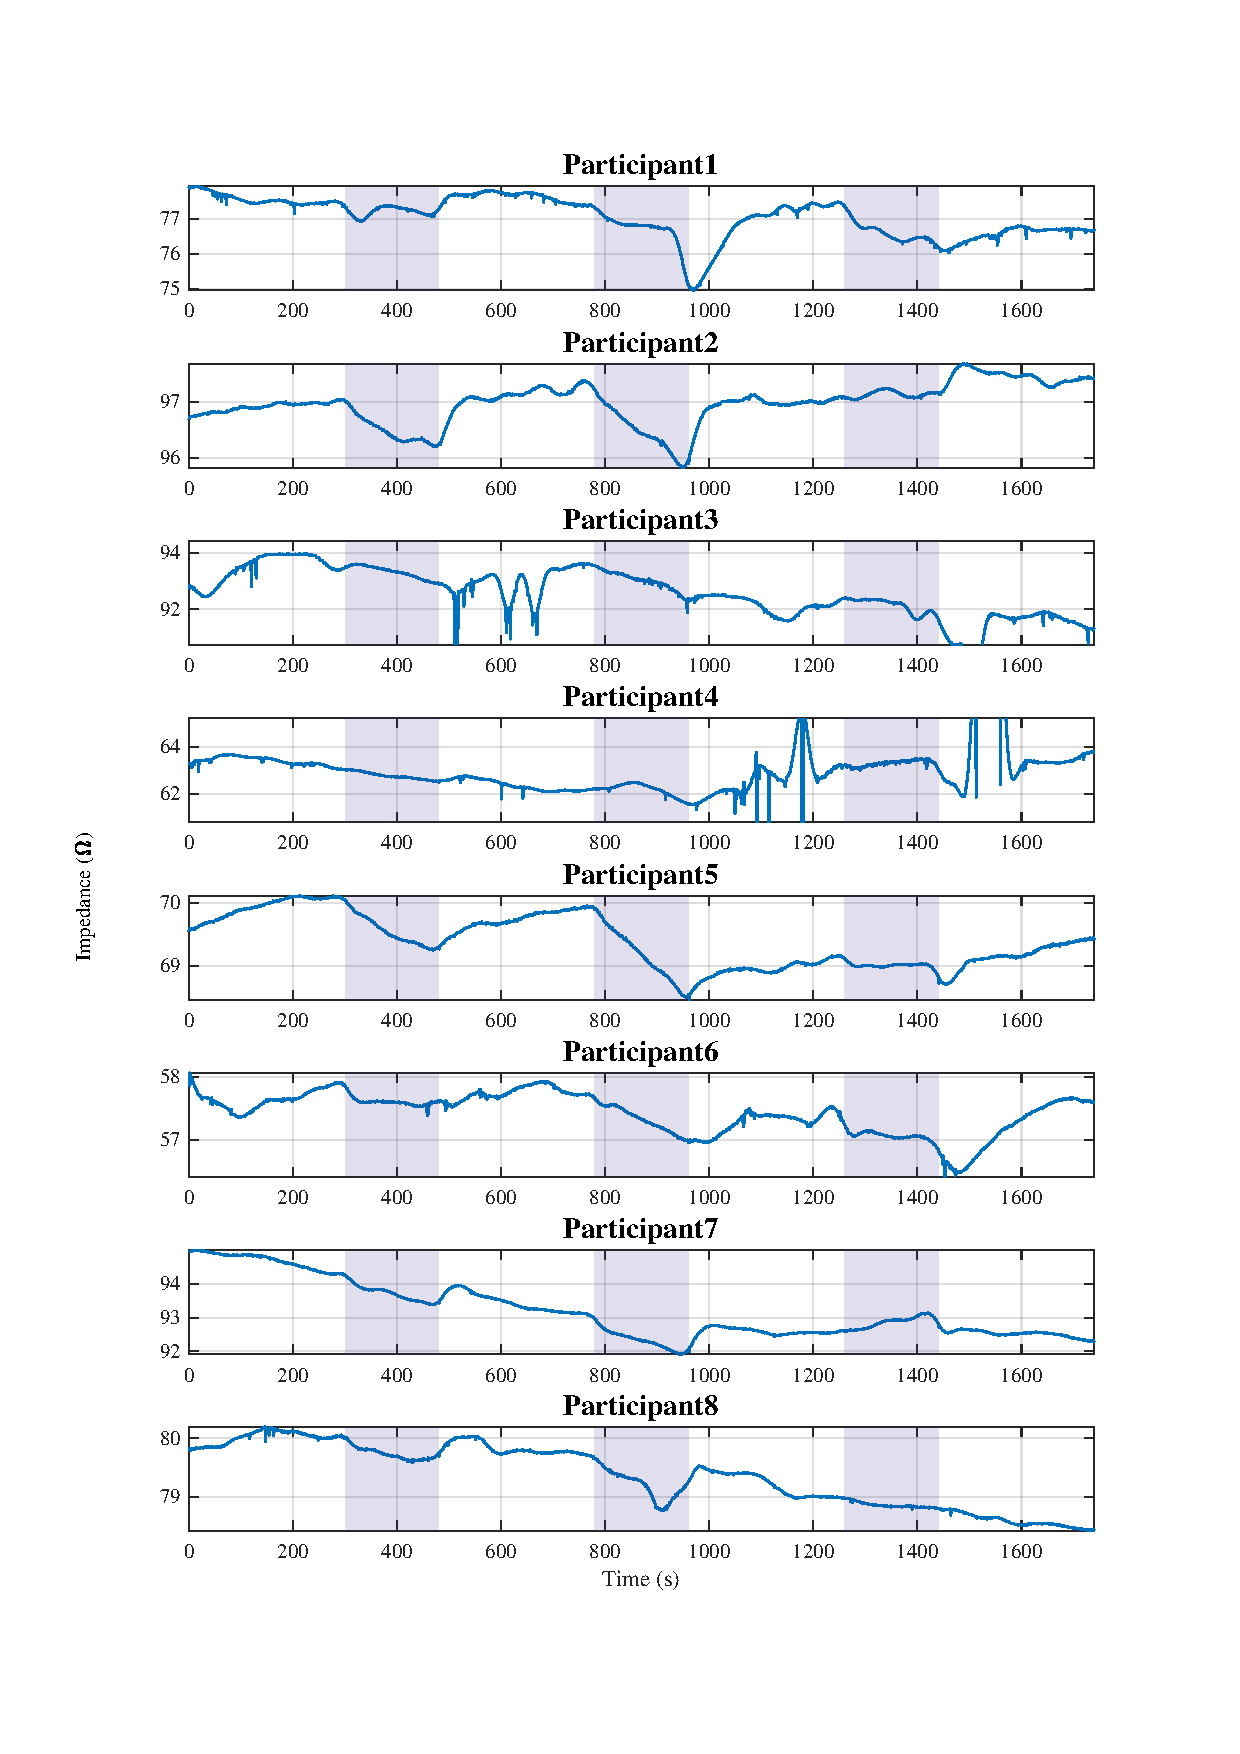
\includegraphics[width=\textwidth,height=\textheight,keepaspectratio]{figure1}    
	\caption{Baseline impedance of all the participants during the study. The shaded areas represent occlusions events.}
	\label{fig:rb:all_participants}
\end{figure}
\todo{This figure is temporary. It needs to be improved by naming axis}

%%********************************** % Section 5.2.1 ******************************************
\subsection{Baseline impedance}
\label{section5.2.1}
The iPG device recorded the impedance during the first five minutes of data logging. 

The device was able to detect the forearm's segment impedance quite remarkably. The values obtained felt within the resistive value estimated by the literature \todo{Find some papers with results about the impedance of the forearms}. The table \ref{tbl:basal_impedace:region1} describes the basal impedance during the first five minutes of data. 

\begin{table}
	\caption{Basal impedance during the first five minutes of data with statistical values.}
	\label{tbl:basal_impedace:region1}
	
	\centering
	\begin{tabular}		
	{
	l
	c
	S[table-format=2.2]@{\,\( \pm \)\,}S[table-format=1.2] %Format for Z+-std
	*{2}{S[table-format=2.2]} 
	}
		\toprule
		              & \textbf{Size} & \multicolumn{2}{c}{\textbf{ $\bar{\textrm{Z}}$ [\si{\ohm}]}} & \textbf{Max [\si{\ohm}]} & \textbf{Min [\si{\ohm}]} \\ \midrule
			Participant 1  &  278  &  77.59  &  0.17  &  78.04  &  77.37\\
			Participant 2  &  295  &  96.97  &  0.09  &  97.17  &  96.76\\
			Participant 3  &  275  &  93.54  &  0.50  &  94.06  &  92.44\\
			Participant 4  &  329  &  63.44  &  0.19  &  63.77  &  63.02\\
			Participant 5  &  288  &  69.97  &  0.17  &  70.20  &  69.56\\
			Participant 6  &  331  &  57.68  &  0.17  &  58.21  &  57.33\\
			Participant 7  &  340  &  94.72  &  0.24  &  95.05  &  94.27\\
			Participant 8  &  353  &  80.04  &  0.11  &  80.30  &  79.82\\ \bottomrule
	\end{tabular} 
\end{table} 

There are different aspects of the geometry that could affect the impedance reading. There have been several studies where has been demonstrated how the distance between electrodes affects readings\todo{Add reference to studies impedance vs. length}. In the current study showed that impedance was influenced by the forearm's circumference, as well as the distance between the potential electrodes. Figure \ref{fig:C_vs_Z} indicates that there is an inverse relation between circumference and impedance. The smallest the forearm's circumference higher the resistivity. On the other hand, there is a direct relation between the distance between the potential electrodes and the resistivity of the segment as depicted in \ref{fig:l_vs_Z}.

In contrast, when comparing total volume measured and mean resistivity of the segment, there is a slight drop of impedance but it is not a clear tendency (see figure \ref{fig:Ve_vs_Z}). As it can be noticed, the data points are scattered depicting a not clear trend. This can be explain as the fat content can affect impedance measurements. As explained by xxx \todo{Add reference about affinity of fat and impedance}, fat is a good conductor of electricity. Hence, fat content does not allow to show a clear tendency in impedance and volume. Nevertheless, in the end the change of volume from the initial basal impedance is going to be caused by the blood streaming trough the vessels.  

\begin{figure*}[t!]
	\centering
	\begin{subfigure}[t]{0.5\textwidth}
		\centering
		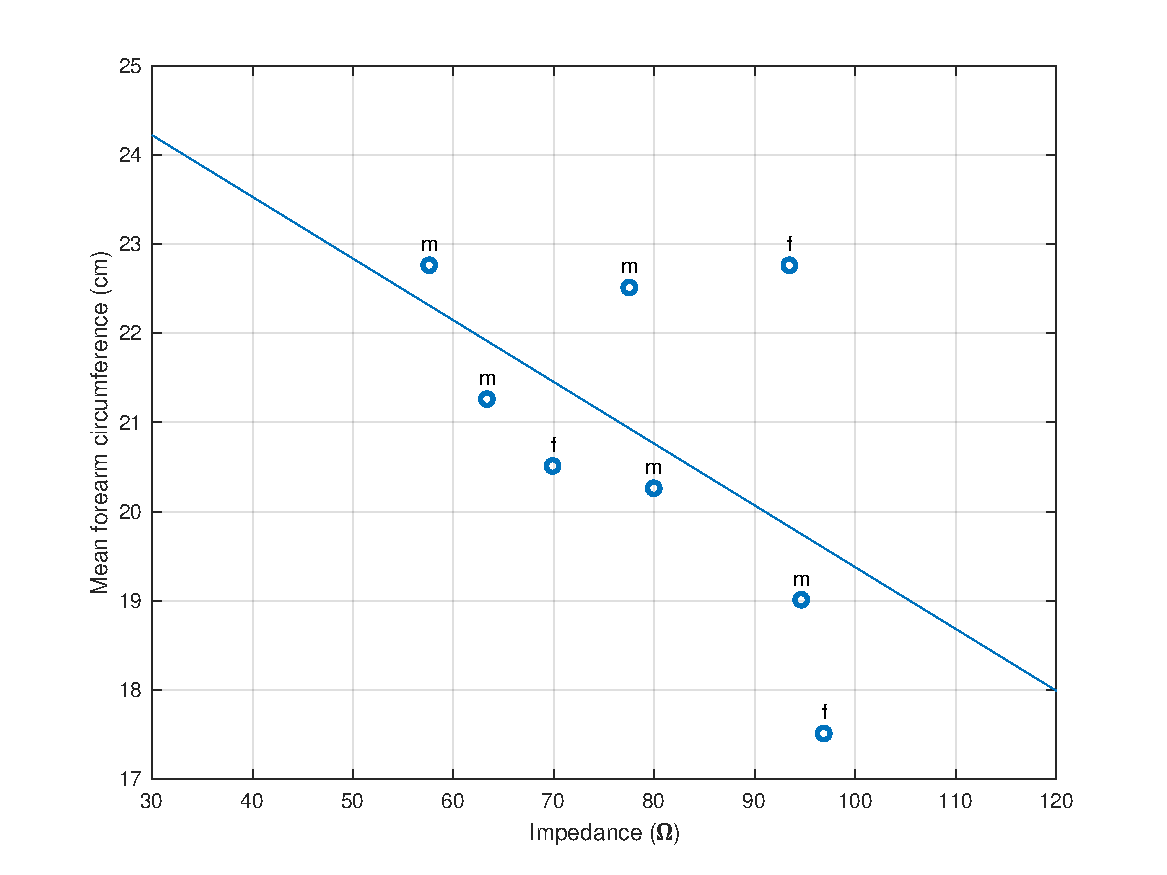
\includegraphics[height=4.5cm]{figure2a}
		\caption{Relationship between forearm circumference and mean basal impedance}
		\label{fig:C_vs_Z}
	\end{subfigure}%
	~ 
	\begin{subfigure}[t]{0.5\textwidth}
		\centering
		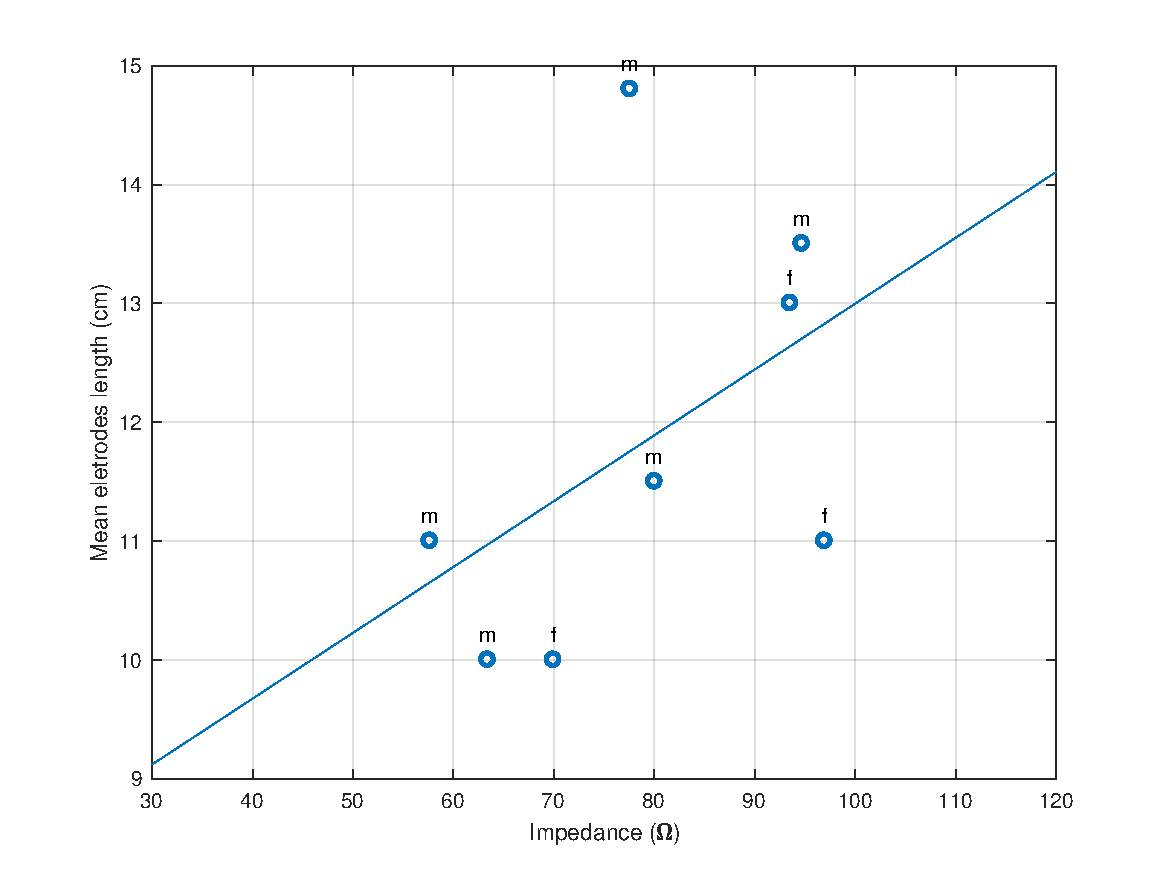
\includegraphics[height=4.5cm]{figure2b}
		\caption{Relationship between distance sensing electrodes and mean basal impedance}
		\label{fig:l_vs_Z}
	\end{subfigure}
	~ 
	\begin{subfigure}[t]{0.5\textwidth}
		\centering
		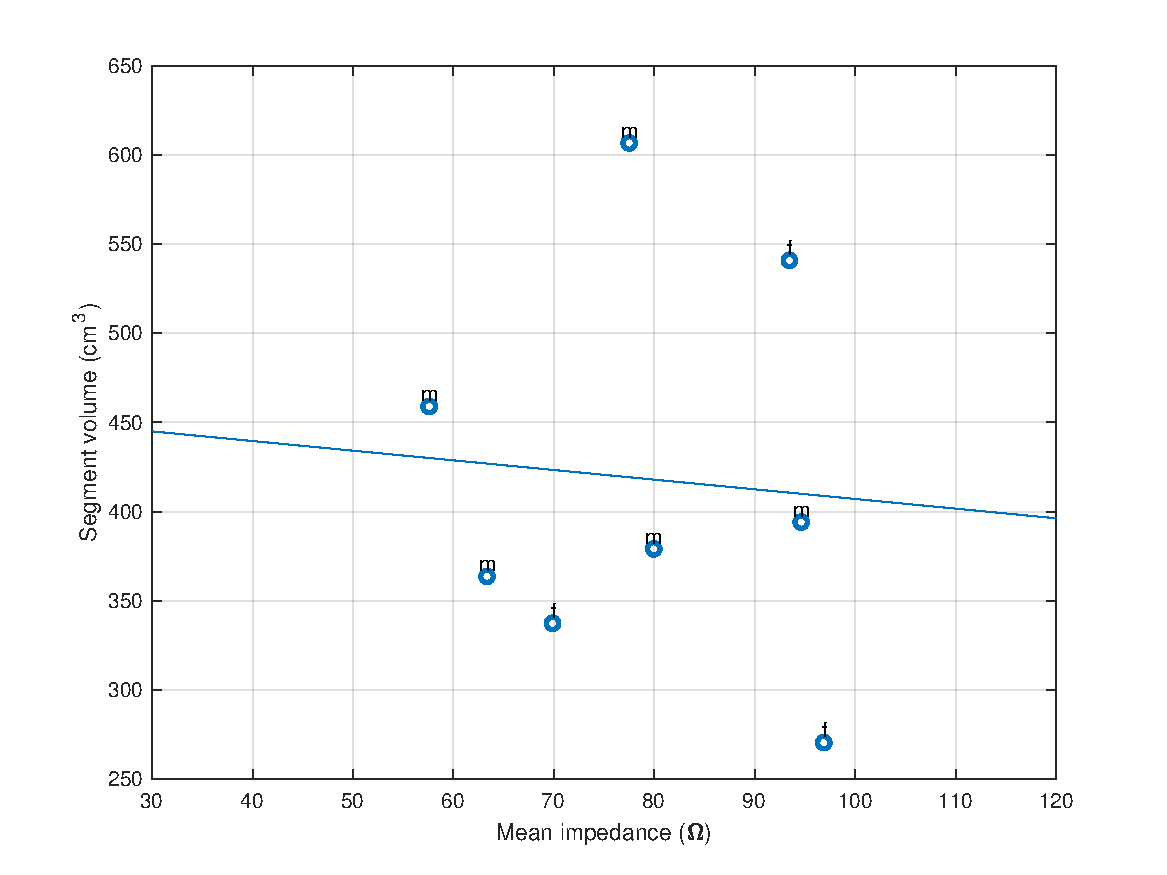
\includegraphics[height=4.5cm]{figure2c}
		\caption{Relation between forearms segment volume and mean basal resistivity}
		\label{fig:Ve_vs_Z}
	\end{subfigure}
	\caption{Relation between circumference, length and total segment's volume and mean basal impedance}
	\label{fig:relation_geometry_vs_impedance}
\end{figure*}


%%********************************** % Section 5.2.2 ******************************************
\subsection{Mean impedance measurement during venous occlusion}
\label{section5.2.2}
During the following three minutes after the impedance, venous occlusion occurred. As it can be seen in figure \ref{fig:rb:all_participants} all the participants experienced a decrease in basal impedance during this time. Most of the helpers presented a linear impedance decrease trend during the occlusion. However, some of the measurements were clearly affected by motion artefact. Participants one and six are an example of this. 

In participant one, resistance fell off immediately the occlusion occurred. Nevertheless, after a minute the patron moved his arm correcting the trend. Then, impedance continued the trend again. Furthermore,  participant six also showed similar response when the arm moved. 

Figure \ref{fig:normalise:venous_occlusion} describes how the impedance behaved during the occlusion for all participants. The graph has been normalised to compare the resistivity reduction.  A linear regression was performed in the data to demonstrate the ratio of change during the occlusion.  

The table \ref{tbl:venous_occlusion:region2} overviews the results obtained from the linear regression. The value $Z_1$ illustrates the value of the impedance as the blockage started and $Z_{end}$ the resistance value at the end of the test.  $\Delta Z$ (mean $-0.632 \Omega \pm0.068\Omega$) is the variation of impedance during the \SI{3}{\minute} that the experiment last.  The slope demonstrates how much resistance is changing during each beat  (mean $-0.00271\Omega\textrm{/s}\pm3.415e^{-6}\Omega\textrm{/s}$). 

\begin{figure}
	\centering
	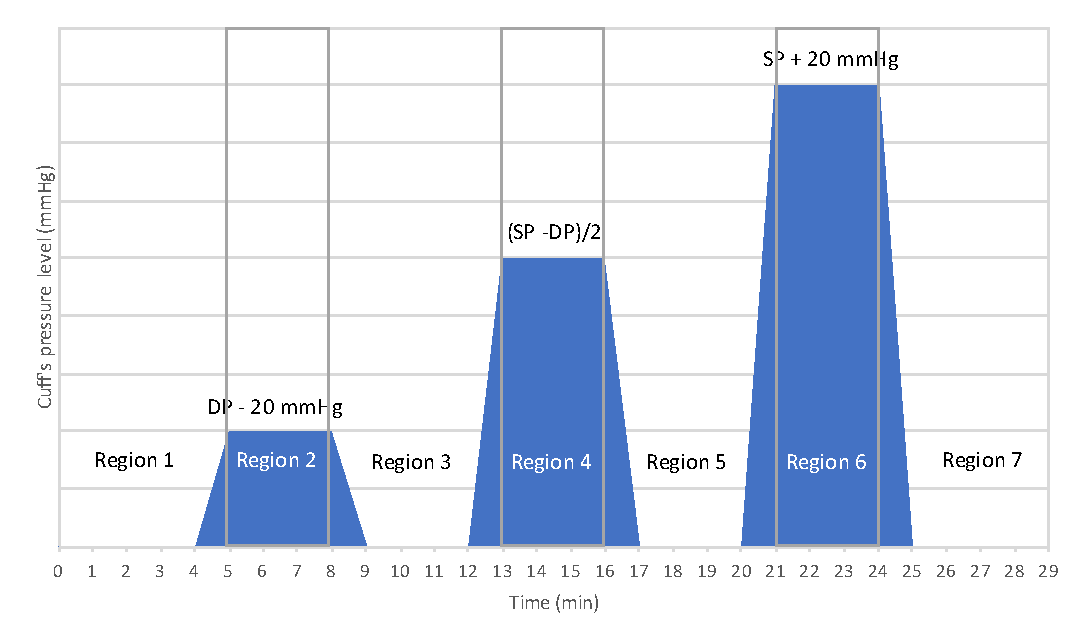
\includegraphics[width=0.9\textwidth,height=0.9\textheight,keepaspectratio]{figure3}    
	\caption{Normalise plot of impedance decrease during venous occlusion.}
	\label{fig:normalise:venous_occlusion}
\end{figure}
\todo{Figure \ref{fig:normalise:venous_occlusion} is temporary. It needs to be improved by naming axis}

\begin{table}[htbp]
	\caption{Linear regression result for all participants during venous occlusion.}
	\label{tbl:venous_occlusion:region2}
	\centering
	\begin{tabu}{lcccccc}
		\toprule
		              & \textbf{Slope [\si{\ohm/\second}]} & \textbf{Intercept [\si{\ohm}]} & \textbf{$R^2$} & \textbf{$Z_1$ [\si{\ohm}]} & \textbf{$Z_{end}$ [\si{\ohm}]} & \textbf{ $\Delta Z$ [\si{\ohm}]} \\ \midrule
		Participant 1  &   0.00057  &  77.02   &     0.037  &  77.49  &  77.18  &  -0.31\\
		Participant 2  &  -0.00395  &  98.09   &     0.867  &  97.16  &  96.21  &  -0.95\\
		Participant 3  &  -0.00421  &  95.01   &     0.917  &  93.47  &  92.89  &  -0.58\\
		Participant 4  &  -0.00296  &  63.96   &     0.920  &  63.22  &  62.61  &  -0.61\\
		Participant 5  &  -0.00427  &  71.26   &     0.936  &  70.10  &  69.27  &  -0.83\\
		Participant 6  &  -0.00085  &  57.96   &     0.322  &  57.98  &  57.57  &  -0.40\\
		Participant 7  &  -0.00427  &  95.42   &     0.934  &  94.33  &  93.34  &  -0.98\\
		Participant 8  &  -0.00173  &  80.43   &     0.752  &  80.07  &  79.68  &  -0.39\\ \bottomrule
	\end{tabu} 
\end{table}

From the statistical analysis displayed can be concluded the following. First, as it was explained before, the slopes from participants 1 and 6 were affected by the motion artefact. Nevertheless, these trends seemed corrected after one minute of recordings (\SI{360}{\second}). Their slopes were quite far away from the mean value (\SI{-0.00271}{\ohm / \second}). On the other hand, the rest of the signals showed a similar trend. \todo{Review this paragraph. It seems to be very similar to the previous one.}


%%********************************** % Section 5.1.3 ******************************************
\subsection{Mean impedance data during arterial occlusion}
\label{section5.2.3}
During partial arterial occlusion, the incoming arterial flow is restricted causing a slow filling of the forearm. Then, total occlusion eliminates the blood inflow under the obstructed section. 

\todo{Check about what happens during partial arterial occlusion. Slow filling of the forearm. This information should also be added to the Medical Background}


%%********************************** % Section 5.1.4 ******************************************
\subsection{Mean impedance data during total occlusion}
\label{section5.2.4}

%%********************************** % Section 5.2 ******************************************
\section{Plethysmography impedance results}
\label{section5.3}

%%********************************** % Section 5.3 ******************************************
\section{Blood flow calculation from baseline signal}
\label{section5.4}


%********************************** % Section 5.3.1 ******************************************
\subsection{Blood flow calculation using venous occlusion plethysmography}
\label{section5.4.1}
Using the method venous occlusion plethysmography is possible to calculate the blood flow in the forearm segment. As it can be seen from figure \ref{fig:blood_flow:venous_occlusion} the data is not dropping in a completely straight line. As a reminder, the occlusion occurred during \SIrange{300}{480}{\second} which is the time lapse showed. There are impedance variations caused by respiration movement contained within the signals, but also some sections are affected by muscle contraction. If the blood flow was computed using point by point method, there would be some discrepancies when the resistivity is increasing. Thus, this will lead to an incorrect reflection of the blood stream. 

As a result, the method described in section xxx was used to calculate the blood flow between decreasing points only. In short, this algorithm finds the peak and valleys of the signal and then computes the blood flow using equation \ref{eq:QL} between those points found. The figure \ref{fig:blood_flow:venous_occlusion} on the left shows the impedance decrease during the occlusion for all participants. The image on also depicts the points from where the algorithm extracted the reference points for its calculations. In this case, the red triangle pointing downwards is equivalent to the base impedance $R_B$ and the black triangle is the ending point of the calculation point. Then $\Delta R / \Delta t$ can be obtained as the difference between these two points in impedance and time. 
\todo{Add a section describing how the data was treated.} 

In the same figure but on the right, it can be noticed the result of the blood flow calculated in units of \si{\ml / \min 100 \ml}. The blue dots indicate the instant blood flow at the end value of $\Delta R$. The orange line indicates the mean blood flow during measurements. Again, participants 1 and 6 flow estimation is affected by movement producing a mean value far from the majority of the data points. Moreover, it is confirmed by examining the results summarised on the table \ref{tbl:blood_flow:region2}. The standard deviation $(\sigma_x)$ is quite far compared to the rest of the participants, as well as the minimum value of the data. Therefore, the results of these two participants clearly cannot be expected to be accurate. However, if the data sample was in a linear section, then the calculated flow will be more in agreement with the expected values. 

From this table can be noticed that the calculated blood flow per \SI{100}{\ml} of tissue for all the participants was in average \SI{-0.855}{\ml / \min 100\ml} $\pm$ \SI{0.344}{\ml/\min 100\ml}. 

\begin{table}[t]
	\caption{Statistics of the blood flow calculated during venous occlusion. All the numbers are in blood flow units \si{\ml/\min 100\ml}, except the column size that is the magnitude of sample.}
	\label{tbl:blood_flow:region2}
	\centering
	\begin{tabular}
		{
			l
			c
			c
			S[table-format=1.3]@{\,\( \pm \)\,}S[table-format=1.3] %Format for Z+-std 
			c
			c
		}
		\toprule
		& \textbf{Size} & \textbf{Median} & \multicolumn{2}{c}{\textbf{Mean}} & \textbf{Max} & \textbf{Min} \\
		& 			    & \small{\si{[\ml/\min 100\ml]}} & \multicolumn{2}{c}{\small{\si{[\ml/\min 100\ml]}}} & \small{\si{[\ml/\min 100\ml]}} & \small{\si{[\ml/\min 100\ml]}} \\\midrule
		Participant 1   & 23   &     -0.808  &   -1.055  &  0.939 &   -0.054   &  -3.955\\
		Participant 2   & 30   &     -0.570  &  -0.575   & 0.272  &  -0.117    & -1.256\\
		Participant 3   & 31   &     -0.600  &  -0.613   & 0.344  &  -0.011    & -1.483\\
		Participant 4   & 34   &     -1.131  &  -1.146   & 0.720  &  -0.016    & -2.979\\
		Participant 5   & 23   &     -0.606  &  -0.611   & 0.345  &  -0.062    & -1.737\\
		Participant 6   & 29   &     -0.710  &  -1.510   & 2.639  &  -0.092    &-10.865\\
		Participant 7   & 25   &     -0.575  &  -0.613   & 0.284  &  -0.025    & -1.141\\
		Participant 8   & 42   &     -0.605  &  -0.716   & 0.530  &  -0.072    & -2.743\\ \bottomrule
	\end{tabular} 
\end{table}

\begin{figure}
	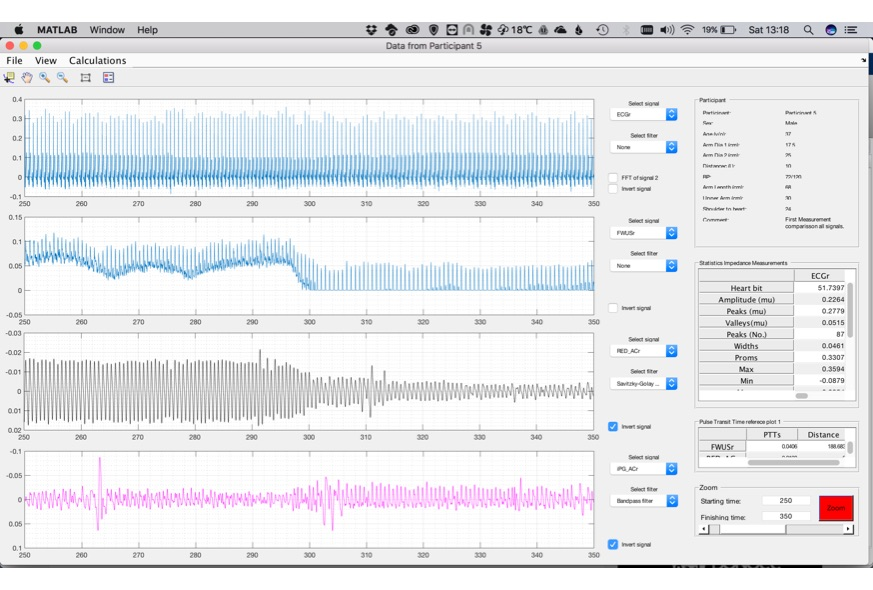
\includegraphics[width=\textwidth,height=\textheight,keepaspectratio,trim={0.5cm 0.5cm 2cm 2cm},clip]{figure4}    
	\caption{Blood flow calculated from venous occlusion plethysmography}
	\label{fig:blood_flow:venous_occlusion}
\end{figure}

%********************************** % Section 5.3.2 ******************************************
\subsection{Blood flow calculation during partial arterial occlusion}
\label{section5.4.2}

%%********************************** % Section 5.4 ******************************************
\section{Blood flow calculation from plethysmography signal}
\label{section5.5}
%********************************** % Section 5.4.1 ******************************************
\subsection{Blood flow beat by beat during baseline}
\label{section5.5.1}

\subsection{Blood flow beat by beat during venous occlusion}
\label{section5.5.2}

\subsection{Blood flow beat by beat during partial arterial occlusion}
\label{section5.5.3}
